\subsubsection{Descripci\'on} 

En ACF los generadores minimales y sus cerrados son elementos esenciales en el ret\'iculo de conceptos  que se obtiene a partir de la relaci\'on binaria de entrada. 

Ser\'ia el equivalente al c\'alculo de las claves minimales. El cerrado de las claves minimales es el conjunto de atributos del dataset. 

Ahora aparecen muchos cerrados y tenemos que calcular sus generadores minimales. Es un problema catalogado como \enquote*{hard} (exponencial en n\'umero de atributos).

Existen algunos algoritmos que  calculan generadores minimales pero no implementados en R y no est\'an basados directamente en l\'ogica. El director del proyecto no ha realizado comparativas en este \'ambito con los otros algoritmos por la no disponibilidad de ellos.



Dados un conjunto de atributos \(M\) y un sistema implicacional \(\Sigma\) sobre \(M\), este algoritmo desarrollado por P. Cordero et al. \cite{LCS} calcula los generadores minimales haciendo uso del concepto de \textit{Labeled Closed Set}, que se basa en que si tenemos un conjunto \(A \subseteq M\), \(A\) es generador minimal si \(X^+_{\Sigma} = A^+_{\Sigma}\) implica que \(X = A\) para todo  \(X \subseteq A\). 

Podemos definir el conjunto de \textit{Labeled Closed Sets} con respecto a \(\Sigma\) como:
\begin{center}
    \(\{<C,mg(C)> | \ C \subseteq M, \ C^+_{\Sigma} = C \}\)\\
    donde \(mg(C) = \{D \subseteq M \ | \ D \ es \ generador \ minimal \ y \ D^+_{\Sigma} = C \}\)
\end{center}

De esta forma, al calcular el conjunto de \textit{Labeled Closed Sets} con el siguiente algoritmo, autom\'aticamente se calculan los generadores minimales.\\

\IncMargin{1em}
\begin{algorithm}[H]
    \SetKwFunction{LabeledClosedSets}
    \SetAlgoLined
    % \LinesNumbered
    \DontPrintSemicolon
    \SetKw{KwOr}{or}
    \KwIn{  
        $M$, the set of all attributes\\
        $ \ \ \ \ \ \ \ \ \ \ \ \ Label$, A structure to build a minimal generator\\
        $ \ \ \ \ \ \ \ \ \ \ \ \ Cicerone$, A structure to build a closed set\\
        $ \ \ \ \ \ \ \ \ \ \ \ \ \Sigma$, an implicational system on $M$
    }
    \KwOut{The set of Labeled Closed Sets}
    \Begin{
        \Repeat{$\Sigma = \Gamma$} {
            \ $\Sigma = \Gamma$\;
            \ $\Gamma = \emptyset$\;
            \For{$A \to B \in \Sigma $}{
                \If{$A \subseteq Cicerone$}{
                    \ $Cicerone := Cicerone \cup {B}$
                }\uElseIf{$B \not\subseteq Cicerone$}{
                    \ $\Gamma := \Gamma \cup \{A \setminus Cicerone \to B \setminus Cicerone\}$
                }
            }
        }
        \ $M := M \setminus Cicerone$\;
        \ $Mnl = \{A \subseteq M \ | \ A \to B \in \Gamma \ for \ some \ B \subseteq M \ and$\; 
        \ $ \ \ \ \ \ \ \ \ \ \ \ \ C \subseteq A \ implies \ C = A \ for \ all \ C \to D \in \Gamma\}$\;
        \ $NC := \{ X \subseteq M \ | \ A \not\subseteq X \ for \ all \ A \in Mnl \}$\;
        \ $LCS := \emptyset$\;
        \ForEach{$X \in NC$}{
            \ $LCS := LCS \cup \{\langle Cicerone \cup X, \{Label \cup X\}\rangle\}$
        }
        \ForEach{$A \in Mnl$}{
            \ $LCS := LCS \cup \LabeledClosedSets{$ M,Label \cup A,Cicerone \cup A, \Gamma $}$
        }
        \Return $LCS$
    }%end beginre
    \caption{LabeledClosedSets algorithm}\label{alg:3}
\end{algorithm}\DecMargin{1em}
\newpage

\subsubsection{C\'odigo} 
\lstinputlisting{r_code/labeled.closed.set.R}
\subsubsection{Ejemplo} 
A continuaci\'on, se muestra un peque\~no ejemplo de ejecuci\'on del algoritmo. Para ello se parte del conjunto de atributos \(M\) y del conjunto de implicaciones \(\Gamma\) que se puede ver en la imagen \ref{fig:lcs_4}.
\begin{figure}[H]
    \centering
    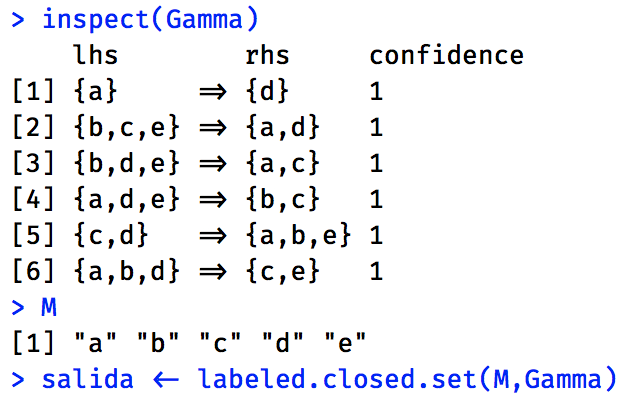
\includegraphics[scale=0.75]{lcs_4}
    \caption{Ejemplo LCS 1}
    \label{fig:lcs_4}
\end{figure} 
\newpage
Aqu\'i se puede ver el resultado:
\begin{figure}[H]
    \centering
    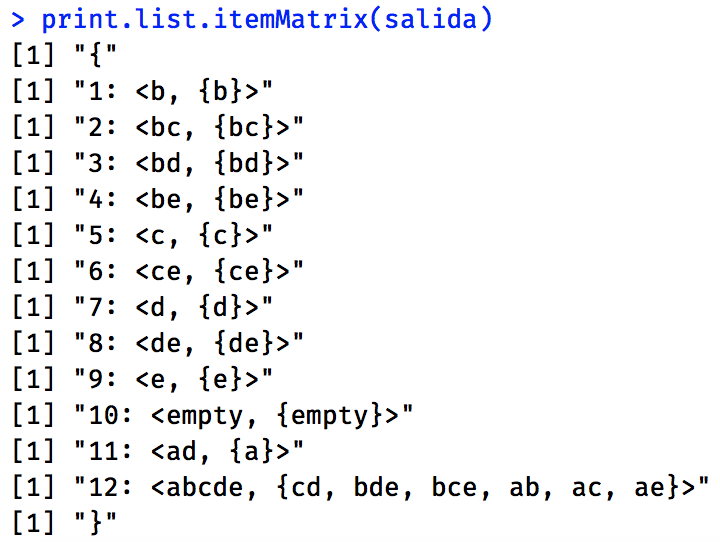
\includegraphics[scale=0.75]{lcs_3}
    \caption{Ejemplo LCS 2}
    \label{fig:lcs_3}
\end{figure}

Como puede verse, por ejemplo, el cerrado 12 tiene como generadores minimales \{cd, bde, bce, ab, ac, ae\}.

Y aqu\'i el resultado que se obtendr\'ia si se usa la otra versi\'on del algoritmo:
\begin{figure}[H]
    \centering
    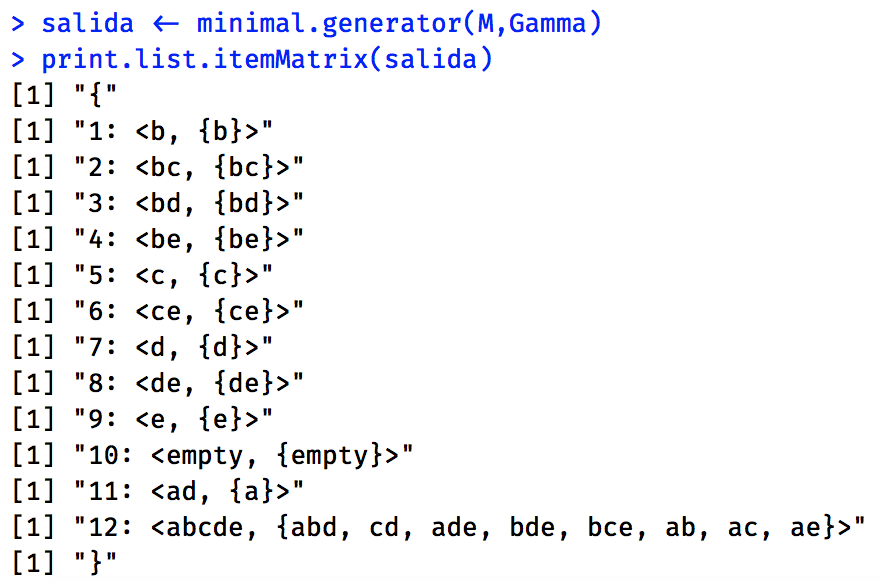
\includegraphics[scale=0.75]{lcs_5}
    \caption{Ejemplo LCS 3}
    \label{fig:lcs_5}
\end{figure}
\newpage
\subsubsection{Comparativa/Versiones} 